% "What the network sees" figure for the A1 poster. Compile on its own, then in the poster:
%   \includegraphics[width=\linewidth]{images/fig_inputs_poster.pdf}
\documentclass[12pt, border=4pt]{standalone}
\usepackage{tikz}
\usetikzlibrary{arrows.meta,positioning,calc,decorations.pathreplacing}
\renewcommand{\familydefault}{\sfdefault}

\definecolor{saclaydk}{RGB}{27,67,32}
\definecolor{mandarine}{RGB}{243,115,32}
\definecolor{vert}{RGB}{140,198,62}
\definecolor{bleu}{RGB}{80,144,205}

\tikzset{
  cell/.style={draw=#1!70!black, fill=#1!45, line width=0.6pt},
  card/.style={draw=#1, fill=#1!10, rounded corners=4pt, line width=1.4pt},
  arr/.style={-{Stealth[length=4mm,width=3mm]}, line width=2pt},
}
\newcommand{\s}{0.36} % cell size

\begin{document}
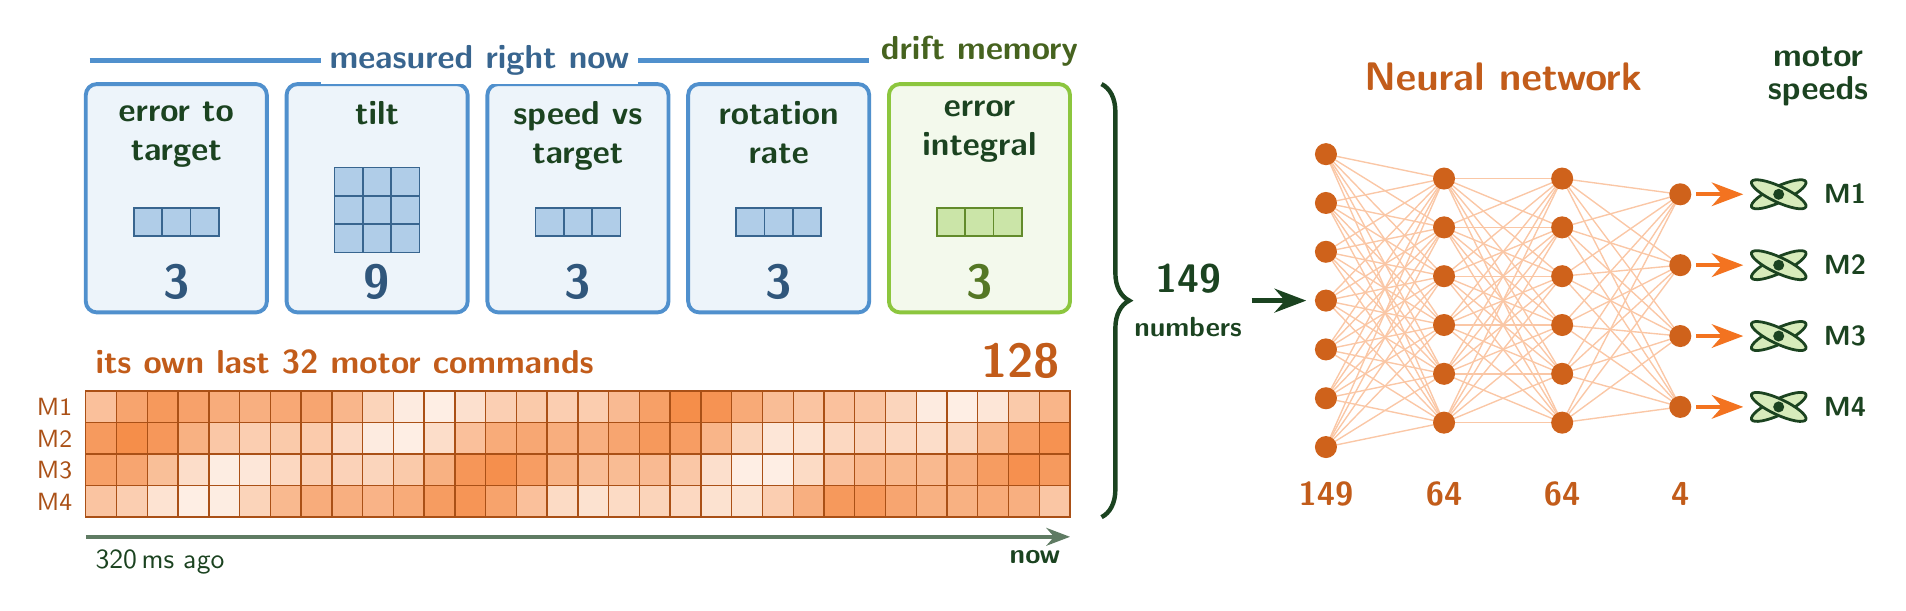
\begin{tikzpicture}
  % ---------- the 5 "right now" groups as cards ----------
  % x-centre / title / count / colour / layout (row = 1x3, grid = 3x3)
  \foreach \x/\ttl/\n/\col/\lay in {
      0/{error to\\target}/3/bleu/row,
      2.55/{tilt}/9/bleu/grid,
      5.1/{speed vs\\target}/3/bleu/row,
      7.65/{rotation\\rate}/3/bleu/row,
      10.2/{error\\integral}/3/vert/row} {
    \draw[card=\col] (\x-1.15,-1.45) rectangle (\x+1.15,1.45);
    \node[align=center, font=\large\bfseries, text=saclaydk, anchor=north] at (\x,1.35) {\ttl};
    \ifx\lay\empty\else\fi
    \node[font=\LARGE\bfseries, text=\col!60!black, anchor=south] at (\x,-1.4) {\n};
  }
  % cells inside the cards
  \foreach \x in {0,5.1,7.65} \foreach \i in {-1,0,1}
    \draw[cell=bleu] (\x+\i*\s-\s/2,-0.3-\s/2) rectangle ++(\s,\s);
  \foreach \i in {-1,0,1} \foreach \j in {-1,0,1}
    \draw[cell=bleu] (2.55+\i*\s-\s/2,-0.15+\j*\s-\s/2) rectangle ++(\s,\s);
  \foreach \i in {-1,0,1}
    \draw[cell=vert] (10.2+\i*\s-\s/2,-0.3-\s/2) rectangle ++(\s,\s);

  % group headers
  \draw[bleu, line width=1.6pt] (-1.1,1.75) -- (8.8,1.75);
  \node[font=\large\bfseries, text=bleu!70!black, fill=white, inner sep=3pt] at (3.85,1.75) {measured right now};
  \node[font=\large\bfseries, text=vert!50!black, anchor=south] at (10.2,1.55) {drift memory};

  % ---------- memory: its own last 32 commands ----------
  \node[anchor=south west, font=\large\bfseries, text=mandarine!80!black] at (-1.15,-2.35)
       {its own last 32 motor commands};
  \node[anchor=south east, font=\LARGE\bfseries, text=mandarine!80!black] at (11.35,-2.4) {128};
  \pgfmathsetmacro{\gw}{12.5/32}
  \foreach \c in {0,...,31} \foreach \r in {0,...,3} {
    \pgfmathtruncatemacro{\v}{max(12, min(85, 45 + 25*sin(\c*23 + \r*70) + 12*sin(\c*61 + \r*20)))}
    \draw[draw=mandarine!70!black, line width=0.5pt, fill=mandarine!\v]
      (-1.15+\c*\gw, -2.45-\r*0.4) rectangle ++(\gw, -0.4);
  }
  \foreach \r/\m in {0/1,1/2,2/3,3/4}
    \node[font=\small, text=mandarine!70!black, anchor=east] at (-1.2,-2.65-\r*0.4) {M\m};
  \draw[-{Stealth[length=3mm]}, line width=1.4pt, saclaydk!70] (-1.15,-4.3) -- (11.35,-4.3);
  \node[anchor=north west, font=\normalsize, text=saclaydk] at (-1.15,-4.35) {320\,ms ago};
  \node[anchor=north east, font=\normalsize\bfseries, text=saclaydk] at (11.35,-4.35) {now};

  % ---------- bracket into the network ----------
  \draw[decorate, decoration={brace, amplitude=10pt}, line width=1.6pt, saclaydk]
    (11.75,1.45) -- (11.75,-4.05) coordinate[midway] (b);
  \node[font=\Large\bfseries, text=saclaydk, align=center] (tot) at (12.85,-1.3) {149\\[-2pt]{\normalsize numbers}};
  \draw[arr, saclaydk] (tot.east) -- (14.35,-1.3);

  % ---------- network ----------
  \def\ny{-1.3}
  \foreach \L/\x/\n/\sp in {0/14.6/7/0.62, 1/16.1/6/0.62, 2/17.6/6/0.62, 3/19.1/4/0.9} {
    \foreach \k in {1,...,\n} \coordinate (N\L-\k) at (\x, {\ny + (\n+1)/2*\sp - \k*\sp});
  }
  \foreach \a/\na/\b/\nb in {0/7/1/6, 1/6/2/6, 2/6/3/4}
    \foreach \i in {1,...,\na} \foreach \j in {1,...,\nb}
      \draw[mandarine!40, line width=0.5pt] (N\a-\i) -- (N\b-\j);
  \foreach \L/\n in {0/7,1/6,2/6,3/4} \foreach \k in {1,...,\n}
    \fill[mandarine!85!black] (N\L-\k) circle (0.14);
  \foreach \x/\lab in {14.6/149, 16.1/64, 17.6/64, 19.1/4}
    \node[font=\large\bfseries, text=mandarine!80!black] at (\x,-3.75) {\lab};
  \node[font=\Large\bfseries, text=mandarine!80!black] at (16.85,1.55) {Neural network};

  % ---------- outputs: 4 propellers ----------
  \foreach \k in {1,...,4} {
    \coordinate (P) at ($(N3-\k)+(1.25,0)$);
    \draw[arr, mandarine, line width=1.4pt] ($(N3-\k)+(0.2,0)$) -- ($(P)+(-0.45,0)$);
    \draw[saclaydk, fill=vert!35, line width=1pt, rotate around={25:(P)}] (P) ellipse (0.38 and 0.1);
    \draw[saclaydk, fill=vert!35, line width=1pt, rotate around={-25:(P)}] (P) ellipse (0.38 and 0.1);
    \fill[saclaydk] (P) circle (0.07);
    \node[anchor=west, font=\normalsize\bfseries, text=saclaydk] at ($(P)+(0.45,0)$) {M\k};
  }
  \node[align=center, font=\large\bfseries, text=saclaydk] at (20.85,1.55) {motor\\[-2pt]speeds};
\end{tikzpicture}
\end{document}
